% Requires \usepackage{graphicx}; paths are relative to the project root.

\begin{figure}[tbp]
  \centering
  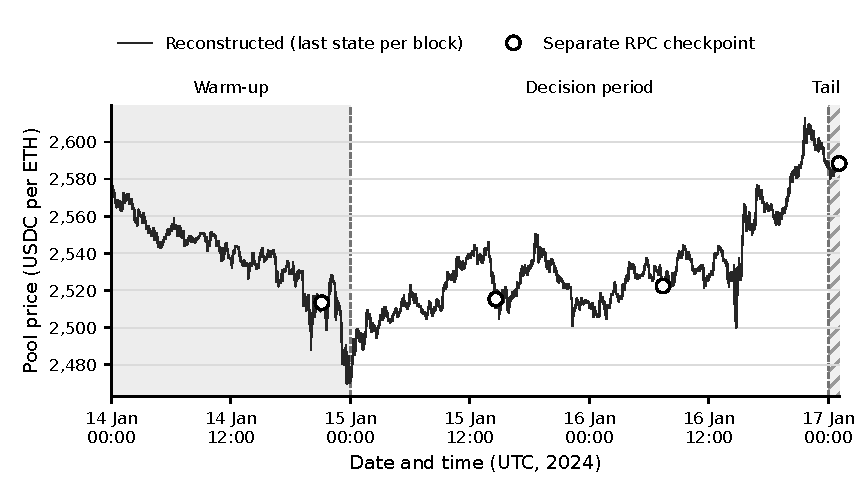
\includegraphics[width=14.5cm]{reports/figures/pilot_pool_reconstruction.pdf}
  \caption{Reconstructed pool price (USDC per ETH) over the captured interval, 14 January to 17 January 2024, including warm-up and the outcome tail. The step line retains the last stored state in each block; dashed boundaries delimit the decision period (15 January to 17 January, exclusive). Circles show separately queried historical end-of-block RPC states at their actual block times. These control states use the same RPC provider as the logs. This price comparison does not itself validate the other state variables or arbitrary counterfactual position outcomes.}
  \label{fig:pilot-pool-reconstruction}
\end{figure}

\begin{figure}[tbp]
  \centering
  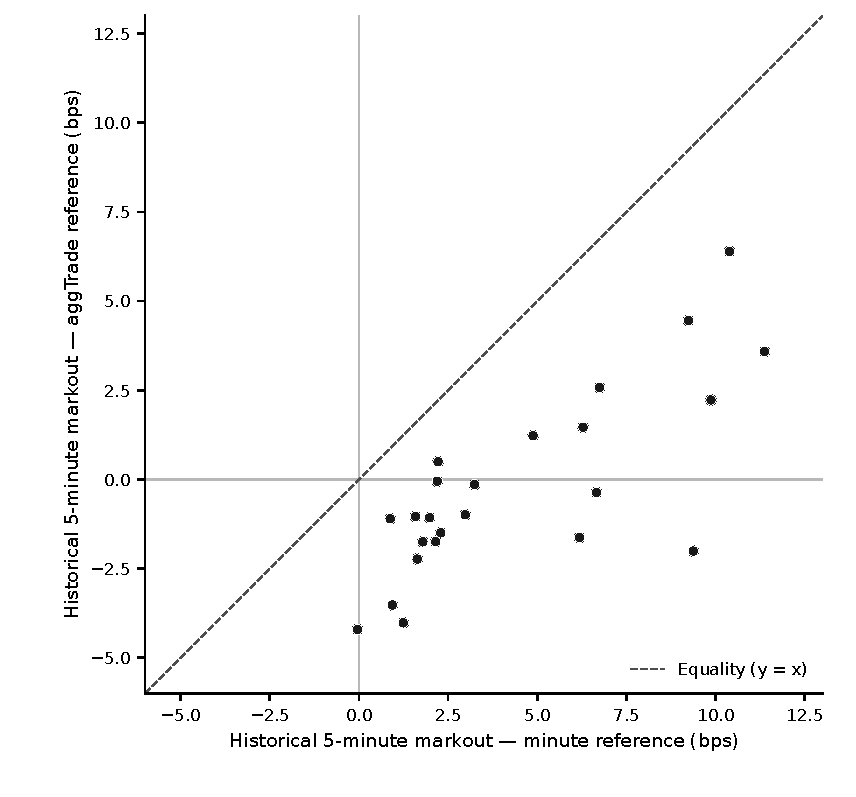
\includegraphics[width=14.5cm]{reports/figures/pilot_markout_resolution.pdf}
  \caption{Historical five-minute markout at 24 hourly decisions on 15 January 2024 (UTC). Each value is the USDC-volume-weighted, signed five-minute reference-price movement over the same 4,527 mature swaps, using identical weights; it is not realized LP loss. Minute and aggTrade references are compared against equality. Finer transaction prices are neither ground truth nor order-book midprices. The figure shows measurement sensitivity, not forecasting performance.}
  \label{fig:pilot-markout-resolution}
\end{figure}
